\documentclass[11pt,a4paper]{article}
\usepackage[margin=2.3cm]{geometry}
\usepackage[T1]{fontenc}\usepackage{lmodern}\usepackage{textcomp}
\usepackage{graphicx,booktabs,float,amsmath,amssymb,xcolor}
\usepackage[hidelinks]{hyperref}
\usepackage{fancyhdr}
\usepackage[numbers,sort]{natbib}
\pagestyle{fancy}\fancyhf{}\rhead{\small Final Report -- MTP}\lhead{\small Multi-Agent LLM Trading on NSE}\cfoot{\thepage}
\setlength{\parskip}{0.45em}\setlength{\parindent}{0pt}
\begin{document}
\begin{titlepage}
\centering
{\large Master Thesis Project -- Final Evaluation Report\par}
\vspace{1.4cm}
{\LARGE\bfseries A Multi-Agent LLM Framework for Explainable\\[0.3em] Algorithmic Trading on NSE-Listed Equities\par}
\vspace{1.4cm}
{\large Vipluv \quad (22MF3IM22)\par}
\vspace{0.4cm}
Department of Industrial \& Systems Engineering\\ Indian Institute of Technology Kharagpur\par
\vspace{0.6cm}
Supervisor: Prof.\ S.\ P.\ Sarmah\par
\vspace{0.6cm}
Track: Financial Analysis / Quantitative Finance\par
\vfill
{\small November 2026}
\end{titlepage}

\begin{abstract}
This project builds and evaluates an explainable multi-agent decision-support system for NSE-listed equities, combining a technical agent based on a peephole LSTM with temporal attention (PLSTM-TAL), an LLM headline-sentiment agent, a market-regime agent, a point-in-time fundamentals agent, a bull/bear LLM debate and a deterministic risk manager. Every configuration is evaluated on a purged, embargoed walk-forward (19,110 out-of-sample decisions, 2018-12-07 to 2026-08-27) under the full Indian delivery cost schedule (about 32 bps round trip), with block-bootstrap confidence intervals, Holm correction and the Deflated Sharpe Ratio. \textbf{No configuration beats Buy-and-Hold} (Buy-and-Hold net Sharpe 0.59; best agent configuration, Tech+Regime, 0.35; no Holm-corrected difference in the agents' favour). The result replicates on a universe three times larger and on data the mid-semester study never saw. What the system does deliver is risk control and auditability: the regime-aware configurations roughly halve maximum drawdown, and a four-part explainability audit shows the rationales are exactly reconstructable, faithful under deletion tests, and -- once a provenance bug the audit itself caught was fixed -- correct about which model produced each number. Because every model, black-box or explainable, sits at chance-level directional accuracy, there is no accuracy--explainability trade-off to pay in this setting.
\end{abstract}
\tableofcontents\newpage
\section{Introduction}
Most published stock-prediction systems emit a single score or direction with no rationale, and are validated on US indices with backtests that ignore transaction costs. Trading desks instead combine several specialists -- technical, fundamental, sentiment, risk -- and argue before committing capital. Indian equities remain comparatively under-studied for LLM-based methods. This project adapts three lines of work (PLSTM-TAL \citep{latif2024}, LLM headline sentiment \citep{lopezlira2023} and multi-agent debate \citep{xiao2024}) to NSE equities and evaluates them under one protocol strict enough that a negative answer is trustworthy.
\subsection{Objectives and final status}
\begin{table}[H]
\centering
\small
\caption{Objectives from the initial and mid-semester reports, and their final status.}\label{tab:status}
\resizebox{\linewidth}{!}{%
\begin{tabular}{p{8.4cm}p{6.6cm}}
\toprule
\textbf{Objective} & \textbf{Status} \\
\midrule
Technical agent: peephole LSTM + temporal attention, next-open direction & Completed (mid-sem); re-trained on 30 names for the final \\
Sentiment agent: LLM scoring of Indian headlines & Completed (mid-sem) \\
Regime agent, bull/bear debate, rule-based risk manager & Completed (mid-sem) \\
Backtest vs Buy-and-Hold, MACD, RSI, KDJ+RSI & Completed (mid-sem); repeated for the final \\
Larger LLM vs local model & Completed: Qwen2.5-3B vs 1.5B (Sec. 5.2) \\
Extended period and universe & Completed: 30 names, data to Nov 2026 (Sec. 5.4) \\
Sentiment around earnings announcements & Completed (Sec. 5.2) \\
Point-in-time fundamentals agent & Completed (Sec. 4.4, 5.3) \\
Cost-aware position sizing & Completed: edge-vs-cost gate + no-trade band (Sec. 4.6) \\
Full ablation re-run; explainability evaluation & Completed (Sec. 5.3, 5.6, 5.7) \\
\bottomrule
\end{tabular}}
\end{table}

\subsection{Contributions}
\begin{itemize}
\item A complete, tested, reproducible multi-agent pipeline for NSE equities (data, five agents, debate, risk manager, cost-aware backtester, live paper-trading demonstration).
\item A strict, pre-registered evaluation: purged and embargoed walk-forward, full Indian cost model, block bootstrap, Holm, Deflated Sharpe. The headline result is negative and is reported as such.
\item A point-in-time fundamentals agent built only from disclosure-lagged annual reports, closing the gap the mid-semester design left open without introducing look-ahead.
\item A measured, not asserted, explainability evaluation (provenance, integrity, reconstruction, deletion faithfulness) and an accuracy--explainability comparison against black-box models.
\end{itemize}
\section{Literature}
\begin{itemize}
\item \textbf{Latif et al.\ (2024)} \citep{latif2024} -- PLSTM-TAL: peephole LSTM with temporal attention for index direction on S\&P 500, FTSE, SSE and Nifty, benchmarked against CNN/LSTM/SVM/RF on seven metrics.
\item \textbf{Lopez-Lira and Tang (2023)} \citep{lopezlira2023} -- LLM headline sentiment predicts next-day returns, concentrated in small caps and negative news; predictability shrinks as LLM adoption rises.
\item \textbf{Xiao et al.\ (2024)} \citep{xiao2024} -- TradingAgents: bull/bear researcher agents and a risk team reach a joint decision; reported to beat Buy-and-Hold, MACD and KDJ+RSI.
\item \textbf{An, Sun and Wang (2022)} \citep{an2022} -- survey of deep RL for trading; reward design, non-stationarity and the sim-to-real gap as open problems.
\item \textbf{Muhammad et al.\ (2024)} \citep{muhammad2024} -- explainable multi-class trend model outperforming random forest.
\end{itemize}
Two things distinguish this study from those papers: the evaluation charges every trade the real Indian cost schedule, and every comparison is tested for statistical significance after correcting for the number of configurations tried. Several published edges do not survive either step here.
\section{Data}
\begin{table}[H]
\centering
\small
\caption{Data used in the final evaluation.}\label{tab:data}
\resizebox{\linewidth}{!}{%
\begin{tabular}{lp{9cm}l}
\toprule
\textbf{Source} & \textbf{Content} & \textbf{Span} \\
\midrule
Prices (core) & 10 liquid NSE large caps, adjusted daily OHLCV, Yahoo Finance & Jan 2015 -- Sep 2026 \\
Prices (extended) & 30 Nifty-50 names (core + 20), separate cache & Jan 2015 -- Nov 2026 \\
Benchmarks & Nifty 50, India VIX & same \\
News & 34,992 headlines (Google News, Indian outlets), noise-filtered & 2016 -- Aug 2026 \\
Fundamentals & Annual P\&L + balance sheet, 30 names (screener.in) & FY2015 -- FY2026 \\
\bottomrule
\end{tabular}}
\end{table}

Two time corrections are applied to news: headlines published after the 15:30 IST close move to the next calendar day, and weekend/holiday dates roll to the next trading session (skipping the second step silently discards 16\% of the corpus). The extended price series are stored in a separate cache because Yahoo's dividend adjustment rewrites past adjusted prices whenever a new dividend is paid; refreshing the original cache in place would have silently moved every mid-semester number.
\section{Methodology}
\subsection{Technical agent (PLSTM-TAL)}
Peephole LSTM cells and a temporal-attention layer are implemented from scratch in PyTorch and trained on 30-day sequences of price/volume/indicator features to predict the probability that the stock rises from the next open to the following open. A $2\times2$ ablation (peephole on/off $\times$ attention on/off), three seeds each, isolates the architecture's contribution. Predictions are seed-averaged; picking the best seed would be selecting on the test set.
\subsection{Sentiment agent}
An instruction-tuned LLM (Qwen2.5-1.5B locally; Qwen2.5-3B for the final comparison) labels each headline \emph{Good}, \emph{Bad} or \emph{Unknown} for the stock. Rather than generating text and parsing it, the backend reads the three labels' first-token logits in one forward pass and renormalises -- deterministic, about 50$\times$ faster, and never unparseable. Daily views average headline scores; confidence falls with headline disagreement and with the model's Unknown mass, and the agent abstains on days without news.
\subsection{Regime agent}
Four causal, equally weighted votes -- price vs its 200-day average, 60-day relative strength vs the Nifty, position in the 52-week range, and (optionally) Nifty momentum -- with confidence cut in high-volatility states.
\subsection{Fundamentals agent (new)}
The mid-semester design deliberately had no fundamental agent because today's ratios inserted into a 2019 decision are look-ahead. The final agent uses only \emph{annual} statements, each treated as unknown until 61 days after the fiscal year end -- one day past SEBI LODR Regulation 33's 60-day deadline for audited results. Using the legal deadline can only make the agent late, never early. Four features (net-profit growth, revenue growth, return on equity, change in ROE) are z-scored \emph{across the universe on each decision date} using only reports public on that date; the stance is half the mean z-score, clipped to $[-1,1]$, at a capped confidence of 0.5 because fundamentals move once a year. Irregular periods from fiscal-year changes (HCLTECH's 9-month 2016, NESTLEIND's 15-month 2024) are recognised: growth is undefined across them and ROE is annualised. Two limitations are stated rather than hidden: the source shows restated rather than as-first-reported figures, and no valuation ratio is used because annual statements do not give a share count consistent with the split-adjusted price series.
\subsection{Debate and the conviction gate}
On contested days a bull and a bear researcher each argue from the agents' findings; the LLM scores the strength of each case by constrained logits, and the net residual moves the score by a fixed 35\% weight (contested debates also cut confidence by 30\%). The mid-semester gate escalated 97.4\% of days because agent stances live on different scales; the conviction gate escalates only when both a confidence-weighted bull and bear stance exceed 0.10. In the final run it escalated 28.9\% of decisions.
\subsection{Trader and risk manager}
The trader takes a confidence-weighted mean of stances (no learned stacker: with about 1,900 test days, a fitted meta-model would fit the test period). The deterministic risk manager applies a confidence floor, volatility targeting (20\% annualised), a drawdown brake and flat limit, a per-name cap of 20\% and a portfolio gross cap of 100\%; idle cash earns a 6\% risk-free rate. Two cost-aware components are new for the final evaluation, both opt-in so the mid-semester numbers reproduce exactly:
\begin{itemize}
\item \textbf{Edge-vs-cost gate}: trade only if score $\times$ confidence $\times$ the stock's typical daily move exceeds the round-trip cost.
\item \textbf{No-trade band} (0.05, fixed in advance at one quarter of the per-name cap): a held position is not resized when the new target is within the band; entries and exits are never banded, so the risk layer can always go flat.
\end{itemize}
\subsection{Evaluation protocol}
Purged, embargoed walk-forward: 3-year training windows, 6-month test windows, a 10-day embargo, 16 folds. Positions are decided at the close of day $t$ and executed at the open of $t+1$, so the return series is open-to-open. Costs follow the 2026 delivery schedule: 0.1\% STT each side, 0.015\% stamp duty on buys, NSE and SEBI charges with GST, and 5 bps slippage -- about 32 bps round trip. Sharpe ratios are excess of 6\%, with stationary block-bootstrap 95\% CIs; paired differences vs Buy-and-Hold are Holm-corrected across all configurations, and the Deflated Sharpe Ratio accounts for the number of strategies tried.
\section{Results}
\subsection{Technical agent}
\begin{table}[H]
\centering
\small
\caption{Architecture ablation, core universe: no variant is distinguishable from a coin flip.}\label{tab:arch}
\resizebox{\linewidth}{!}{%
\begin{tabular}{lrrrr}
\toprule
\textbf{Architecture} & \textbf{Accuracy (mean \$\textbackslash{}pm\$ sd)} & \textbf{AUC} & \textbf{MCC} & \textbf{p vs chance} \\
\midrule
LSTM & 0.5045 $\pm$ 0.0019 & 0.5049 & 0.0076 & 0.21 \\
LSTM-TAL & 0.5024 $\pm$ 0.0005 & 0.5017 & 0.0056 & 0.51 \\
PLSTM-TAL & 0.4998 $\pm$ 0.0048 & 0.5008 & 0.0007 & 0.96 \\
PLSTM & 0.4996 $\pm$ 0.0003 & 0.4999 & -0.0018 & 0.90 \\
\bottomrule
\end{tabular}}
\end{table}

Re-trained on the extended 30-name universe (58,620 out-of-sample rows per run), the result is the same: LSTM-TAL 0.4999 $\pm$ 0.0019 (3 seeds); PLSTM-TAL 0.4987 $\pm$ 0.0006 (3 seeds). Tripling the cross-section does not create a directional edge.
\subsection{Sentiment: earnings announcements and model size}
About 10\% of headlines are results/earnings news (a keyword classifier whose matches were checked by reading a random sample). Earnings sessions are genuinely information-rich: the mean absolute next-day move is 133 bps against 126 bps on other news days ($t=2.18$, $p=0.029$).
\begin{table}[H]
\centering
\small
\caption{Full corpus, Qwen2.5-1.5B: predictability of debiased daily sentiment, earnings vs other sessions. Holm p is adjusted across every cell of the sentiment study.}\label{tab:earn}
\resizebox{\linewidth}{!}{%
\begin{tabular}{lrrrrrrr}
\toprule
\textbf{Subset} & \textbf{Horizon} & \textbf{n} & \textbf{IC} & \textbf{IC p} & \textbf{Holm p} & \textbf{Pos-Neg (bps)} & \textbf{Hit rate} \\
\midrule
all news days & 1 day & 15,190 & +0.0016 & 0.841 & 1.000 & -0.1 & 50.1\% \\
all news days & 5 days & 15,158 & -0.0001 & 0.987 & 1.000 & -2.7 & 49.9\% \\
earnings days & 1 day & 1,803 & -0.0273 & 0.247 & 1.000 & -15.0 & 48.7\% \\
earnings days & 5 days & 1,796 & -0.0282 & 0.232 & 1.000 & -36.0 & 48.6\% \\
non-earnings days & 1 day & 13,387 & +0.0055 & 0.526 & 1.000 & +2.0 & 50.2\% \\
non-earnings days & 5 days & 13,362 & +0.0034 & 0.691 & 1.000 & +2.1 & 50.1\% \\
\bottomrule
\end{tabular}}
\end{table}

On the full corpus, where an earnings session's tone is diluted by all other headlines that day, sentiment predicts neither the next day nor the next five: every information coefficient is indistinguishable from zero. The picture sharpens when the daily view is built mainly from the earnings headlines themselves (the matched sample below).
\begin{figure}[H]
\centering
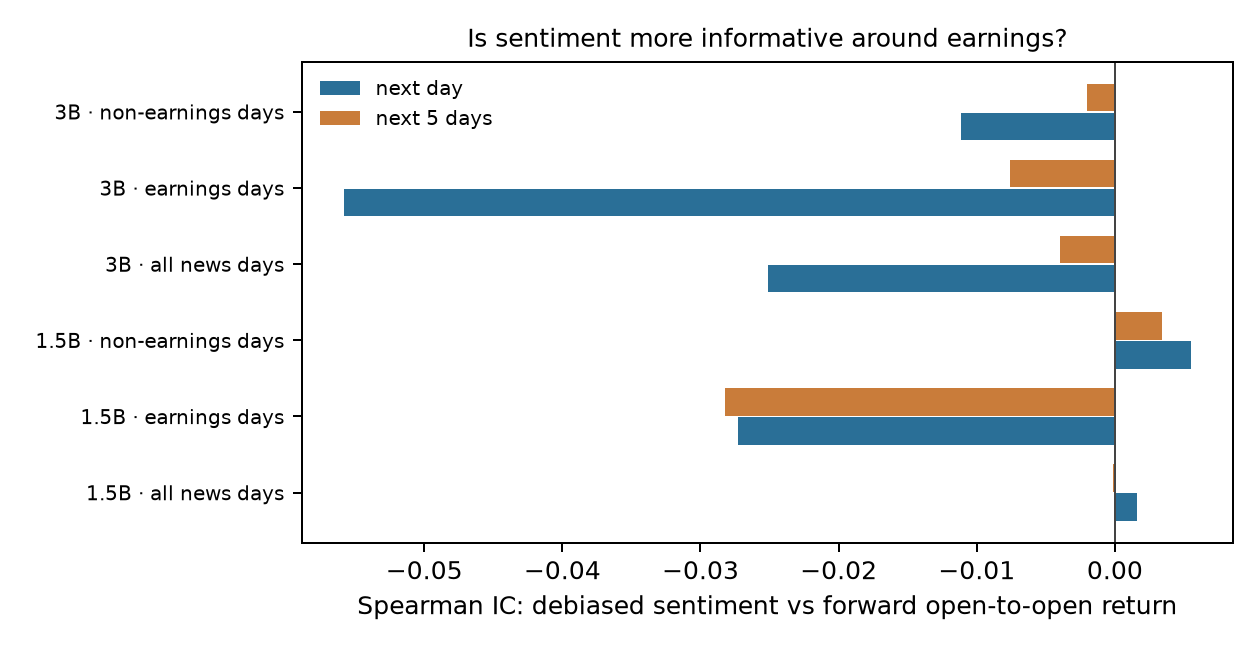
\includegraphics[width=0.8\linewidth]{earnings_ic.png}
\caption{Information coefficient of debiased sentiment by model, subset and horizon.}
\end{figure}

\begin{table}[H]
\centering
\small
\caption{Label distributions. The 1.5B model's bullish prior is the documented 3:1 Good:Bad ratio.}\label{tab:labels}
\resizebox{\linewidth}{!}{%
\begin{tabular}{lrrrrr}
\toprule
\textbf{Model} & \textbf{Headlines} & \textbf{Good} & \textbf{Bad} & \textbf{Unknown} & \textbf{Good:Bad} \\
\midrule
Qwen2.5-1.5B (full corpus) & 34,992 & 48.1\% & 14.5\% & 37.4\% & 3.31 \\
Qwen2.5-1.5B (matched) & 10,240 & 49.9\% & 15.9\% & 34.3\% & 3.14 \\
Qwen2.5-3B (matched) & 10,240 & 19.8\% & 11.7\% & 68.5\% & 1.70 \\
\bottomrule
\end{tabular}}
\end{table}

Both models scored the identical 10,240 headlines (every earnings headline plus a random sample of the rest) with the identical prompt and constrained-logit scoring. They agree on 60.3\% of labels (Cohen's $\kappa=0.39$). The larger model is far less bullish -- Good:Bad 1.70 against 3.14 -- and far more willing to say a headline is not about the stock's price (Unknown 68.5\% vs 34.3\%).
\begin{table}[H]
\centering
\small
\caption{Qwen2.5-1.5B vs Qwen2.5-3B on matched headlines: next-day predictability. Holm p is adjusted across the comparison family.}\label{tab:llm}
\resizebox{\linewidth}{!}{%
\begin{tabular}{lrrrrrrr}
\toprule
\textbf{Model} & \textbf{Subset} & \textbf{Score} & \textbf{n views} & \textbf{IC} & \textbf{Holm p} & \textbf{Pos-Neg (bps)} & \textbf{Hit rate} \\
\midrule
Qwen2.5-1.5B & all & raw & 6480 & -0.0293 & 0.072 & -13.2 & 49.2\% \\
Qwen2.5-1.5B & all & debiased & 6480 & -0.0187 & 0.132 & -8.4 & 48.4\% \\
Qwen2.5-1.5B & earnings & raw & 1803 & -0.0835 & 0.003 & -26.4 & 48.1\% \\
Qwen2.5-1.5B & earnings & debiased & 1803 & -0.0576 & 0.072 & -21.4 & 47.6\% \\
Qwen2.5-3B & all & raw & 6480 & -0.0421 & 0.004 & -18.0 & 48.5\% \\
Qwen2.5-3B & all & debiased & 6480 & -0.0251 & 0.086 & -13.9 & 49.2\% \\
Qwen2.5-3B & earnings & raw & 1803 & -0.0850 & 0.002 & -37.3 & 46.4\% \\
Qwen2.5-3B & earnings & debiased & 1803 & -0.0558 & 0.072 & -27.1 & 47.9\% \\
\bottomrule
\end{tabular}}
\end{table}

\begin{figure}[H]
\centering
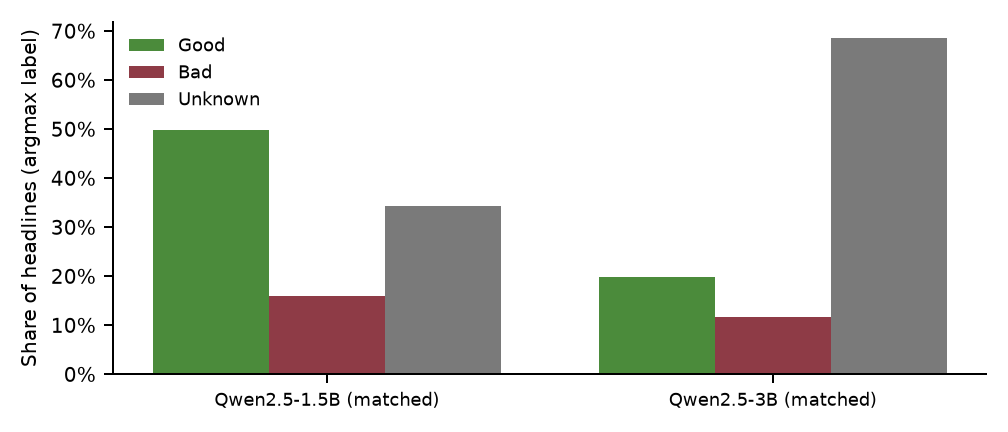
\includegraphics[width=0.7\linewidth]{llm_labels.png}
\caption{Label shares on matched headlines.}
\end{figure}

\textbf{A reversal, not a continuation.} On earnings sessions, the raw tone of the earnings headlines predicts the next open-to-open return with the \emph{opposite} sign for both models (IC -0.084, -0.085; Holm-adjusted $p$ 0.003, 0.002): positive-tone results are followed by underperformance, the positive-minus-negative tercile spread being -26, -37 bps. Because the system trades only from the open after a headline is actionable, the initial reaction has already happened; what remains is a partial overshoot that corrects. Three qualifications keep this from being an edge: it does not survive the causal debiasing step (Holm $p$ 0.072, 0.072); the spread is a long-short figure of the same order as the 32 bps round-trip cost; and it is the opposite of what a long-only sentiment agent that buys on good news assumes -- which is part of why adding sentiment never helped in the ablation. It is the direction Lopez-Lira and Tang's own result would predict for a market in which the news is already priced.
Doubling the model size changes \emph{how} headlines are labelled -- a much weaker bullish prior -- but not the conclusion: neither model's tone is a usable long-only signal. Within the compute available here, a larger model is not the missing ingredient.
\subsection{Full ablation, core universe}
All configurations share 19,110 decisions (2018-12-07 to 2026-08-27), the same execution and the same cost model. The mid-semester configurations reproduce their published Sharpe ratios to within 0.004 (the residual is the price-snapshot correction described in Section 6), so every new component is measured against effectively the same baseline.
\begin{table}[H]
\centering
\footnotesize
\caption{Core ablation (10 names). Sharpe is net of costs and excess of 6\% risk-free.}\label{tab:core}
\resizebox{\linewidth}{!}{%
\begin{tabular}{lrrrrrrrr}
\toprule
\textbf{Strategy} & \textbf{Sharpe net} & \textbf{Sharpe gross} & \textbf{CAGR} & \textbf{MaxDD} & \textbf{Vol} & \textbf{Turnover/yr} & \textbf{Exposure} & \textbf{Holm p vs B\textbackslash{}\&H} \\
\midrule
Buy\&Hold & 0.59 & 0.59 & 16.4\% & -38.6\% & 19.0\% & 0.1x & 100\% & -- \\
RSI(14) & 0.43 & 0.47 & 12.3\% & -39.8\% & 17.0\% & 4.2x & 60\% & 0.818 \\
Tech+Regime & 0.35 & 0.58 & 10.1\% & -20.7\% & 13.8\% & 20.4x & 86\% & 0.818 \\
Regime+Fund+Band & 0.28 & 0.47 & 9.0\% & -22.2\% & 13.5\% & 16.0x & 84\% & 0.598 \\
Tech+Regime+Fund & 0.24 & 0.50 & 8.5\% & -23.2\% & 14.1\% & 23.2x & 88\% & 0.588 \\
Regime+Fund & 0.21 & 0.48 & 8.2\% & -23.2\% & 14.1\% & 23.6x & 88\% & 0.588 \\
Tech+Sent+Regime & 0.17 & 0.66 & 7.5\% & -25.0\% & 14.4\% & 43.4x & 90\% & 0.414 \\
All4+Debate(conviction) & 0.14 & 0.60 & 7.0\% & -24.7\% & 15.2\% & 43.1x & 93\% & 0.088 \\
Full+Debate(conviction) & 0.14 & 0.62 & 7.0\% & -27.2\% & 14.6\% & 43.6x & 91\% & 0.208 \\
Tech+Regime+Fund+CostAware+Band & 0.14 & 0.37 & 6.5\% & -5.3\% & 3.7\% & 5.2x & 7\% & 0.818 \\
Tech+Sent+Regime+Fund & 0.04 & 0.59 & 5.5\% & -25.0\% & 14.6\% & 49.4x & 91\% & 0.141 \\
MACD & 0.02 & 0.46 & 5.0\% & -29.9\% & 15.5\% & 42.9x & 78\% & 0.387 \\
KDJ+RSI & -0.34 & 0.24 & 0.1\% & -39.3\% & 14.2\% & 50.8x & 34\% & 0.006 \\
Tech-only & -0.41 & -0.27 & 3.1\% & -25.4\% & 6.3\% & 5.5x & 16\% & 0.088 \\
All4+CostAware+Band & -0.52 & 0.20 & 4.2\% & -5.1\% & 3.2\% & 14.1x & 7\% & 0.208 \\
MeanReversion & -1.41 & 0.68 & -18.1\% & -79.6\% & 17.3\% & 223.4x & 76\% & 0.000 \\
\bottomrule
\end{tabular}}
\end{table}

\begin{figure}[H]
\centering
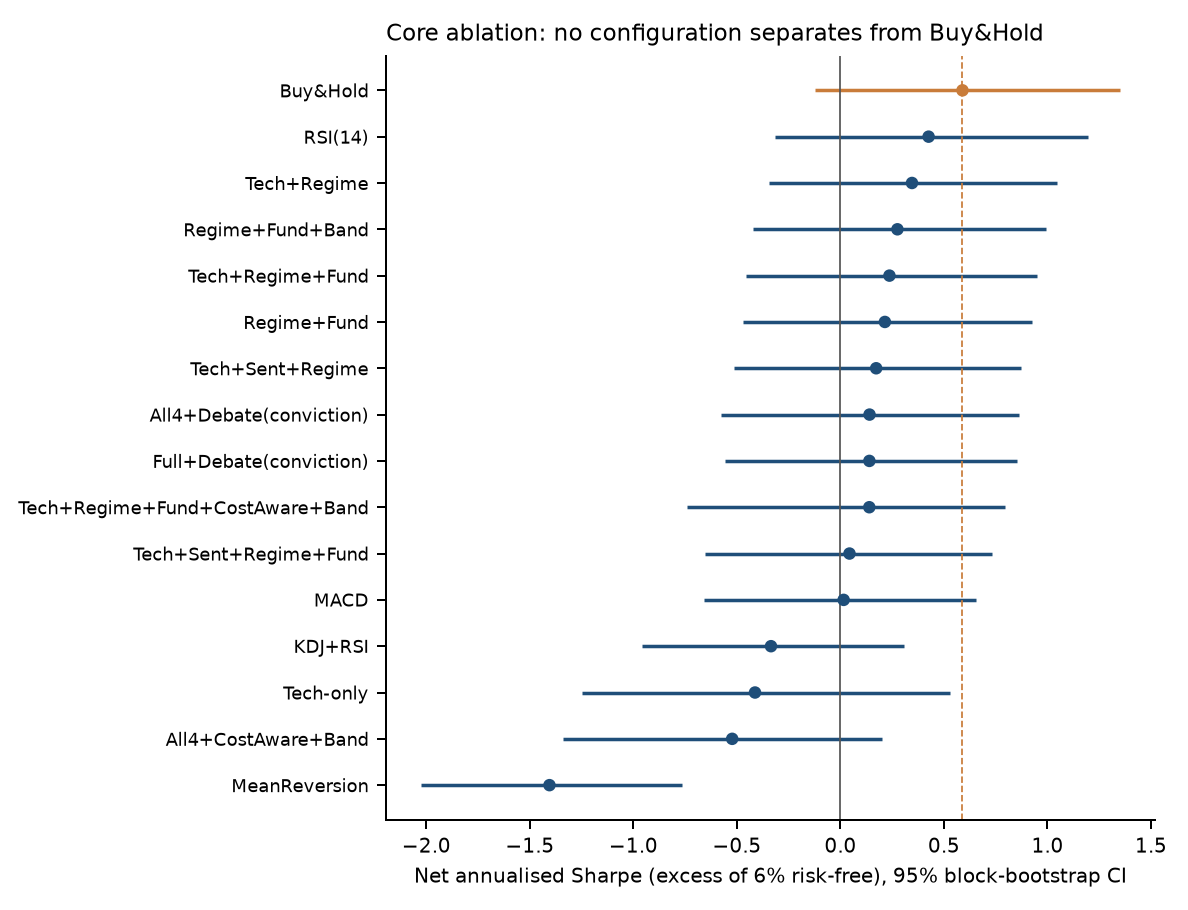
\includegraphics[width=0.92\linewidth]{forest_core.png}
\caption{Net Sharpe with 95\% block-bootstrap CIs (core universe). The dashed line is Buy-and-Hold.}
\end{figure}

\begin{figure}[H]
\centering
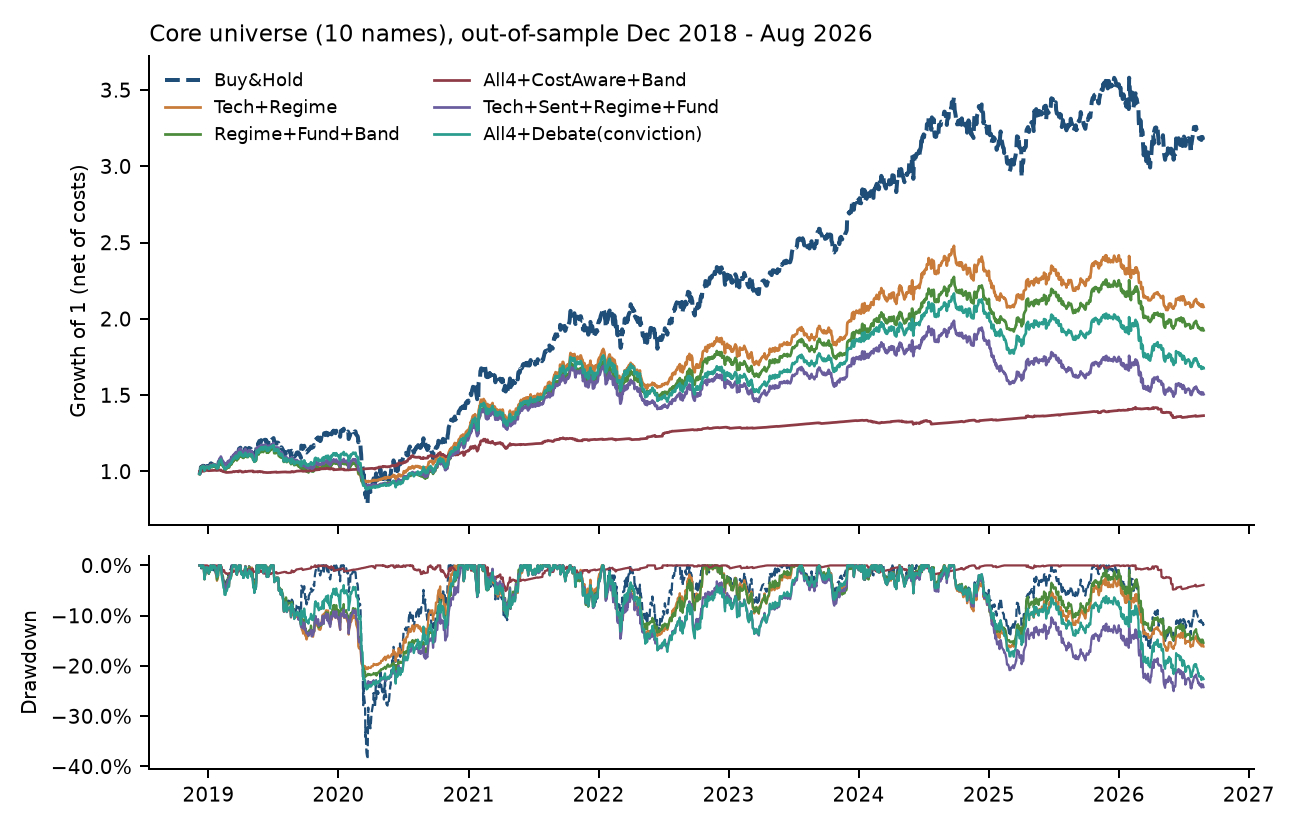
\includegraphics[width=0.92\linewidth]{equity_core.png}
\caption{Equity and drawdown, core universe, net of costs.}
\end{figure}

\paragraph{What each new component did.}
\begin{itemize}
\item \textbf{Fundamentals} lower Sharpe when added to Tech+Regime (0.35 $\to$ 0.24) and do not rescue the sentiment configuration (0.17 $\to$ 0.04). Annual quality/growth rankings among ten large caps carry no short-horizon information.
\item \textbf{The no-trade band} cuts turnover (23.6x $\to$ 16.0x a year) and lifts Sharpe (0.21 $\to$ 0.28) -- the only component that helps, and it helps by trading less, not by predicting better.
\item \textbf{The edge-vs-cost gate} works as designed and exposes the core finding: almost no signal clears the 32 bps hurdle, so the book is invested only 7\% of the time. Its small drawdown (-5.1\%) is the drawdown of cash, and its Calmar ratio should be read that way.
\item \textbf{Conviction-gated debate}: 0.14 without fundamentals, 0.14 with them.
\end{itemize}
\subsection{Extended universe and fresh data}
The extended experiment re-trains the technical agent on 30 names and runs to 2026-11-04 (58,620 decisions). No news corpus exists for the 20 added names, so it tests the technical, regime and fundamentals agents and the risk layer.
\begin{table}[H]
\centering
\footnotesize
\caption{Extended universe (30 names). Same protocol and costs.}\label{tab:ext}
\resizebox{\linewidth}{!}{%
\begin{tabular}{lrrrrrrrr}
\toprule
\textbf{Strategy} & \textbf{Sharpe net} & \textbf{Sharpe gross} & \textbf{CAGR} & \textbf{MaxDD} & \textbf{Vol} & \textbf{Turnover/yr} & \textbf{Exposure} & \textbf{Holm p vs B\textbackslash{}\&H} \\
\midrule
Buy\&Hold & 0.74 & 0.74 & 18.5\% & -34.3\% & 17.2\% & 0.1x & 100\% & -- \\
RSI(14) & 0.66 & 0.74 & 17.5\% & -38.5\% & 18.2\% & 9.3x & 93\% & 0.558 \\
Regime+Fund+Band & 0.36 & 0.57 & 10.2\% & -25.1\% & 13.0\% & 16.3x & 88\% & 0.038 \\
Tech+Regime & 0.35 & 0.67 & 10.4\% & -24.7\% & 14.6\% & 29.1x & 98\% & 0.031 \\
Tech+Regime+Fund & 0.25 & 0.57 & 8.8\% & -27.8\% & 14.7\% & 28.9x & 98\% & 0.006 \\
Regime+Fund & 0.25 & 0.56 & 8.7\% & -27.8\% & 14.7\% & 29.0x & 98\% & 0.006 \\
MACD & 0.23 & 0.91 & 8.5\% & -29.1\% & 16.5\% & 70.1x & 98\% & 0.086 \\
Tech-only & 0.09 & 0.29 & 6.4\% & -7.7\% & 5.6\% & 7.2x & 15\% & 0.198 \\
Tech+Regime+Fund+CostAware+Band & 0.06 & 0.39 & 6.1\% & -17.8\% & 8.3\% & 17.4x & 28\% & 0.086 \\
KDJ+RSI & -0.92 & 0.20 & -10.8\% & -64.2\% & 17.1\% & 119.4x & 66\% & 0.000 \\
MeanReversion & -1.97 & 0.85 & -26.5\% & -91.8\% & 17.8\% & 311.2x & 96\% & 0.000 \\
\bottomrule
\end{tabular}}
\end{table}

\begin{figure}[H]
\centering
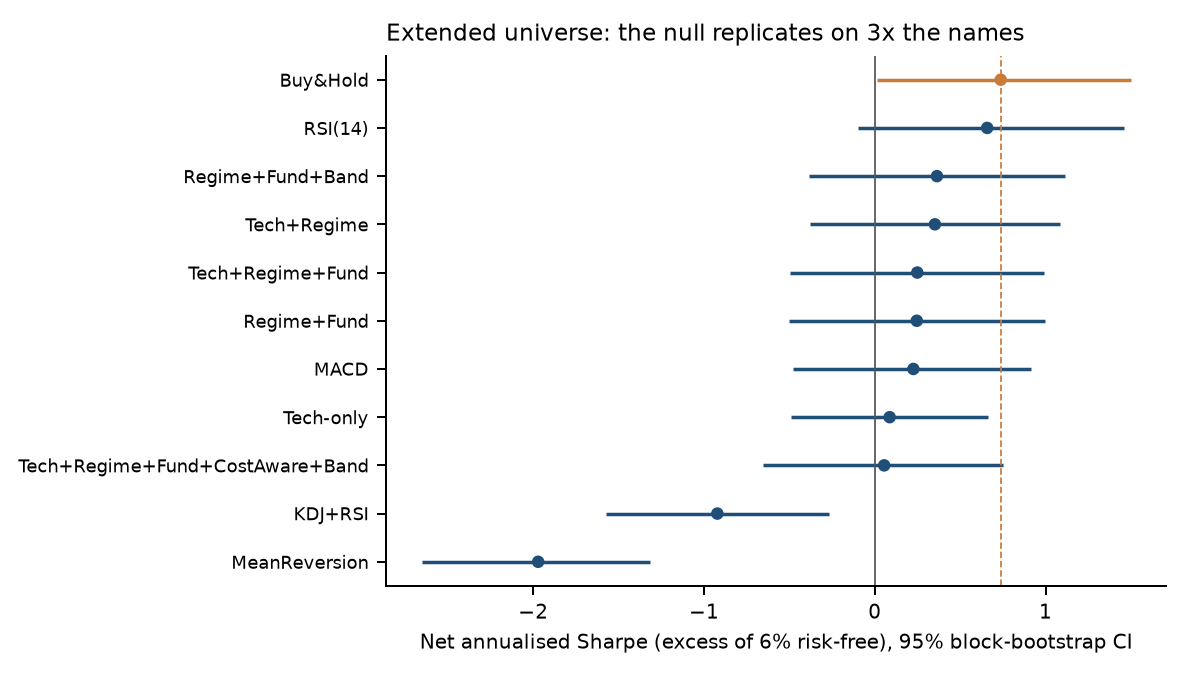
\includegraphics[width=0.92\linewidth]{forest_extended.png}
\caption{Net Sharpe with 95\% CIs, extended universe.}
\end{figure}

\begin{figure}[H]
\centering
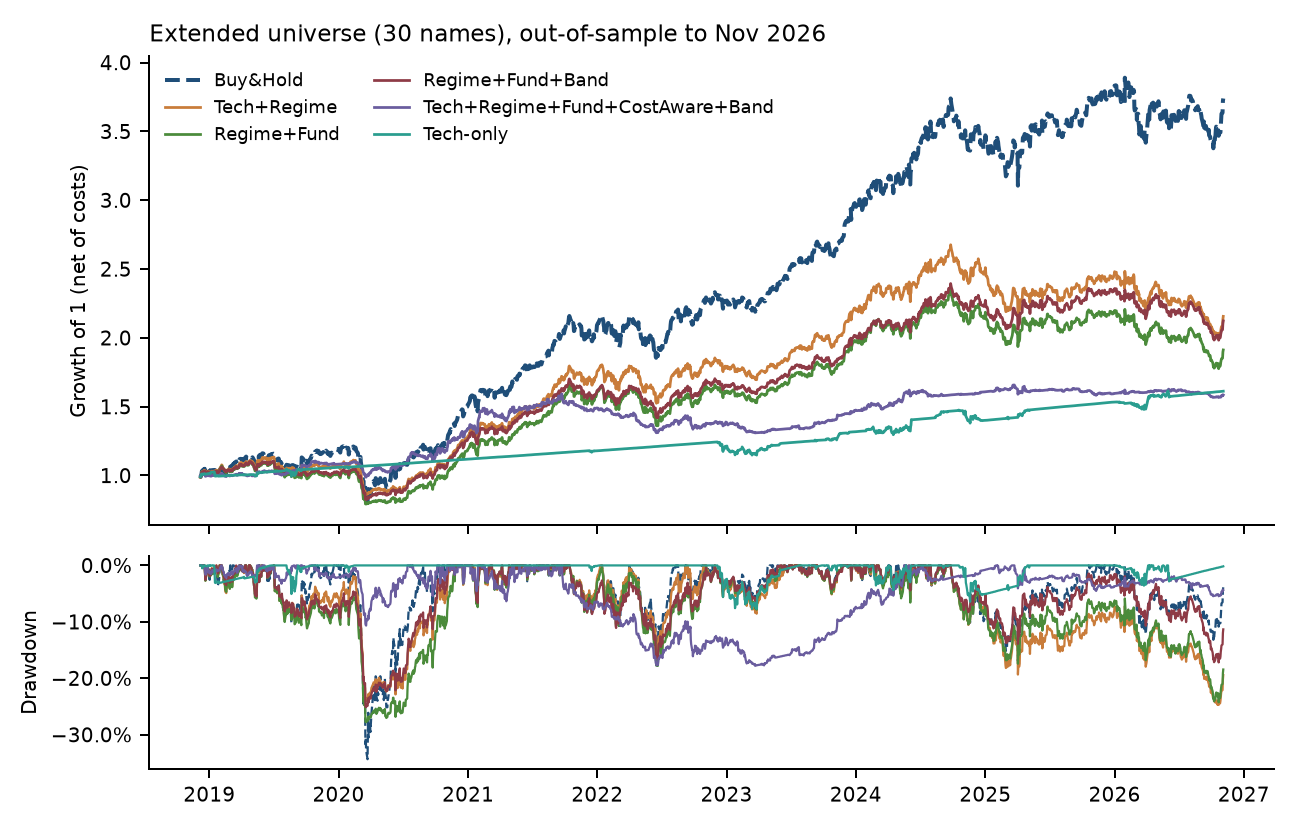
\includegraphics[width=0.92\linewidth]{equity_extended.png}
\caption{Equity and drawdown, extended universe.}
\end{figure}

Buy-and-Hold's Sharpe on the wider universe is 0.74; the ordering of configurations replicates, and no configuration improves on Buy-and-Hold. With three times the cross-section the test gains power, and the negative result sharpens: 4 agent configurations (Regime+Fund+Band, Tech+Regime, Tech+Regime+Fund, Regime+Fund) are now \emph{significantly worse} than Buy-and-Hold after Holm correction. The null result is not an artefact of a ten-stock universe.
\begin{table}[H]
\centering
\small
\caption{Truly fresh holdout: Sep--Nov 2026, data that did not exist at the mid-semester review. Too short for inference; reported for completeness.}\label{tab:fresh}
\resizebox{\linewidth}{!}{%
\begin{tabular}{lrrr}
\toprule
\textbf{Strategy} & \textbf{Days} & \textbf{Return} & \textbf{Max DD} \\
\midrule
Tech-only & 44 & 1.02\% & 0.00\% \\
Tech+Regime & 44 & -2.49\% & -9.46\% \\
Tech+Regime+Fund & 44 & -3.58\% & -10.90\% \\
Regime+Fund & 44 & -3.60\% & -10.92\% \\
Regime+Fund+Band & 44 & -2.52\% & -9.36\% \\
Tech+Regime+Fund+CostAware+Band & 44 & -0.57\% & -2.07\% \\
Buy\&Hold & 44 & 3.15\% & -7.34\% \\
MACD & 44 & 2.31\% & -8.97\% \\
RSI(14) & 44 & 4.57\% & -6.13\% \\
KDJ+RSI & 44 & -4.71\% & -10.04\% \\
MeanReversion & 44 & -2.80\% & -9.40\% \\
\bottomrule
\end{tabular}}
\end{table}

\subsection{Risk control in stressed markets}
Using the mid-semester definition -- every day on which the Nifty's trailing 60-day return is below $-10\%$ (94 trading days, almost all in the 2020 COVID crash) -- the regime-aware configurations protect capital exactly when it matters:
\begin{table}[H]
\centering
\small
\caption{Maximum drawdown over crash-regime days only (core universe).}\label{tab:crash}
\resizebox{\linewidth}{!}{%
\begin{tabular}{lr}
\toprule
\textbf{Strategy} & \textbf{Max drawdown in crash regime} \\
\midrule
MeanReversion & -24.1\% \\
RSI(14) & -24.0\% \\
KDJ+RSI & -24.0\% \\
Buy\&Hold & -23.6\% \\
MACD & -9.9\% \\
Tech-only & -9.2\% \\
All4+Debate(conviction) & -8.8\% \\
Full+Debate(conviction) & -7.6\% \\
Tech+Sent+Regime+Fund & -5.2\% \\
Tech+Sent+Regime & -4.7\% \\
Regime+Fund+Band & -3.3\% \\
Tech+Regime+Fund & -2.7\% \\
Regime+Fund & -2.5\% \\
Tech+Regime & -1.1\% \\
Tech+Regime+Fund+CostAware+Band & -0.5\% \\
All4+CostAware+Band & -0.4\% \\
\bottomrule
\end{tabular}}
\end{table}

The same pattern holds over calendar windows (March--June 2020; January--June 2022), reported in \texttt{results/final/core/subperiods.csv}. The overlay trades upside for downside protection, and over the full period that trade loses on net -- a different finding from ``no effect''.
\subsection{Explainability evaluation}
Explainability is treated as a testable property. Four checks run over every logged decision:
\begin{enumerate}
\item \textbf{Provenance}: does the rationale name the model that actually produced its numbers?
\item \textbf{Integrity}: do the stated action, score and per-agent stances equal the logged values?
\item \textbf{Reconstruction}: can the score be recomputed from the logged opinions alone?
\item \textbf{Deletion faithfulness}: removing the agent named most influential should flip the decision far more often than removing another agent.
\end{enumerate}
\begin{table}[H]
\centering
\footnotesize
\caption{Audit-trail integrity across every decision log.}\label{tab:audit}
\resizebox{\linewidth}{!}{%
\begin{tabular}{lrrrrrr}
\toprule
\textbf{Run} & \textbf{Configuration} & \textbf{Provenance} & \textbf{Stances match} & \textbf{Score match} & \textbf{Reconstructable} & \textbf{Words/rationale} \\
\midrule
mid-sem & Full+Debate & 0\% & 100.00\% & 100.00\% & 100.00\% & 108 \\
mid-sem & Tech+Regime & 0\% & 100.00\% & 100.00\% & 100.00\% & 83 \\
mid-sem & Tech+Sent+Regime & 0\% & 100.00\% & 100.00\% & 100.00\% & 96 \\
mid-sem & Tech+Sentiment & 0\% & 100.00\% & 100.00\% & 100.00\% & 57 \\
mid-sem & Tech-only & 0\% & 100.00\% & 100.00\% & 100.00\% & 43 \\
final-core & All4+CostAware+Band & 100\% & 100.00\% & 100.00\% & 100.00\% & 123 \\
final-core & All4+Debate(conviction) & 100\% & 100.00\% & 100.00\% & 100.00\% & 133 \\
final-core & Full+Debate(conviction) & 100\% & 100.00\% & 100.00\% & 100.00\% & 97 \\
final-core & Regime+Fund+Band & n/a & 100.00\% & 100.00\% & 100.00\% & 93 \\
final-core & Regime+Fund & n/a & 100.00\% & 100.00\% & 100.00\% & 87 \\
final-core & Tech+Regime+Fund+CostAware+Band & 100\% & 100.00\% & 100.00\% & 100.00\% & 110 \\
final-core & Tech+Regime+Fund & 100\% & 100.00\% & 100.00\% & 100.00\% & 115 \\
final-core & Tech+Regime & 100\% & 100.00\% & 100.00\% & 100.00\% & 83 \\
final-core & Tech+Sent+Regime+Fund & 100\% & 100.00\% & 100.00\% & 100.00\% & 128 \\
final-core & Tech+Sent+Regime & 100\% & 100.00\% & 100.00\% & 100.00\% & 96 \\
final-core & Tech-only & 100\% & 100.00\% & 100.00\% & 100.00\% & 43 \\
final-extended & Regime+Fund+Band & n/a & 100.00\% & 100.00\% & 100.00\% & 96 \\
final-extended & Regime+Fund & n/a & 100.00\% & 100.00\% & 100.00\% & 90 \\
final-extended & Tech+Regime+Fund+CostAware+Band & 100\% & 100.00\% & 100.00\% & 100.00\% & 110 \\
final-extended & Tech+Regime+Fund & 100\% & 100.00\% & 100.00\% & 100.00\% & 118 \\
final-extended & Tech+Regime & 100\% & 100.00\% & 100.00\% & 100.00\% & 85 \\
final-extended & Tech-only & 100\% & 100.00\% & 100.00\% & 100.00\% & 43 \\
\bottomrule
\end{tabular}}
\end{table}

The provenance check found a real defect: all 19,110 rationales in the mid-semester logs credited PLSTM-TAL for predictions produced by LSTM-TAL, because the runner never told the technical agent which model it was wrapping. Every number was correct; the explanation was not. It is fixed, and the final logs pass at 100\%. An explainability claim that had only been asserted would never have caught this.
\begin{table}[H]
\centering
\small
\caption{Deletion faithfulness: decision flips when the top-attributed vs a random other agent is removed.}\label{tab:del}
\resizebox{\linewidth}{!}{%
\begin{tabular}{lrrrr}
\toprule
\textbf{Configuration} & \textbf{n} & \textbf{Flip: delete top agent} & \textbf{Flip: delete other agent} & \textbf{McNemar p} \\
\midrule
All4+CostAware+Band & 19,110 & 41.6\% & 3.2\% & $<10^{-6}$ \\
All4+Debate(conviction) & 19,110 & 37.4\% & 3.4\% & $<10^{-6}$ \\
Full+Debate(conviction) & 19,102 & 52.7\% & 0.5\% & $<10^{-6}$ \\
Regime+Fund+Band & 19,080 & 46.8\% & 3.2\% & $<10^{-6}$ \\
Regime+Fund & 19,080 & 46.8\% & 3.2\% & $<10^{-6}$ \\
Tech+Regime+Fund+CostAware+Band & 19,110 & 47.3\% & 2.0\% & $<10^{-6}$ \\
Tech+Regime+Fund & 19,110 & 47.3\% & 2.1\% & $<10^{-6}$ \\
Tech+Regime & 19,080 & 71.3\% & 0.0\% & $<10^{-6}$ \\
Tech+Sent+Regime+Fund & 19,110 & 41.6\% & 3.3\% & $<10^{-6}$ \\
Tech+Sent+Regime & 19,102 & 52.6\% & 0.6\% & $<10^{-6}$ \\
\bottomrule
\end{tabular}}
\end{table}

\begin{figure}[H]
\centering
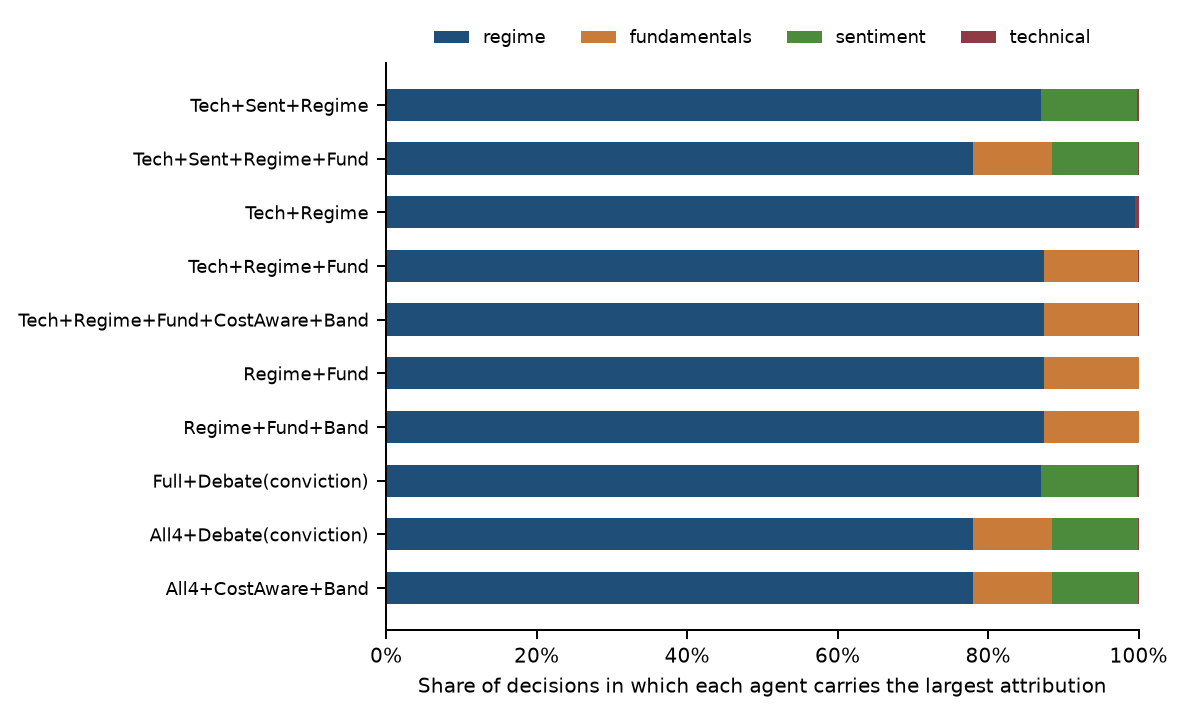
\includegraphics[width=0.85\linewidth]{decisive_agent.png}
\caption{Which agent carries the largest attribution in each decision.}
\end{figure}

The attributions are faithful, and what they reveal matters more than any Sharpe ratio: the regime agent is the decisive input in the large majority of decisions, the technical model almost never. The explanations show directly that the multi-agent system behaves as a trend filter with a risk overlay -- which is exactly why it protects capital in crashes and gives up return in rallies.
\subsection{The accuracy--explainability trade-off}
Explainability is scored on a five-criterion rubric of binary, checkable properties: E1 per-decision natural-language rationale; E2 exact additive attribution; E3 explicit abstention; E4 risk overrides in the audit trail; E5 adversarial bull-vs-bear argument.
\begin{table}[H]
\centering
\small
\caption{Directional accuracy vs explainability score.}\label{tab:trade}
\resizebox{\linewidth}{!}{%
\begin{tabular}{lrrr}
\toprule
\textbf{Model} & \textbf{Class} & \textbf{Directional accuracy} & \textbf{Explainability (0--5)} \\
\midrule
LSTM (black box) & black-box & 0.5045 & 0 \\
LSTM-TAL (black box) & black-box & 0.5024 & 0 \\
PLSTM-TAL (black box) & black-box & 0.4998 & 0 \\
PLSTM (black box) & black-box & 0.4996 & 0 \\
GBM (black box) & black-box & 0.4998 & 0 \\
Tech+Regime & agents+risk & 0.5016 & 4 \\
Tech+Regime+Fund & agents+risk & 0.5006 & 4 \\
Tech+Sent+Regime+Fund & agents+risk & 0.5029 & 4 \\
All4+CostAware+Band & agents+risk & 0.5029 & 4 \\
Full+Debate(conviction) & agents+risk+debate & 0.5024 & 5 \\
All4+Debate(conviction) & agents+risk+debate & 0.5055 & 5 \\
\bottomrule
\end{tabular}}
\end{table}

\begin{figure}[H]
\centering
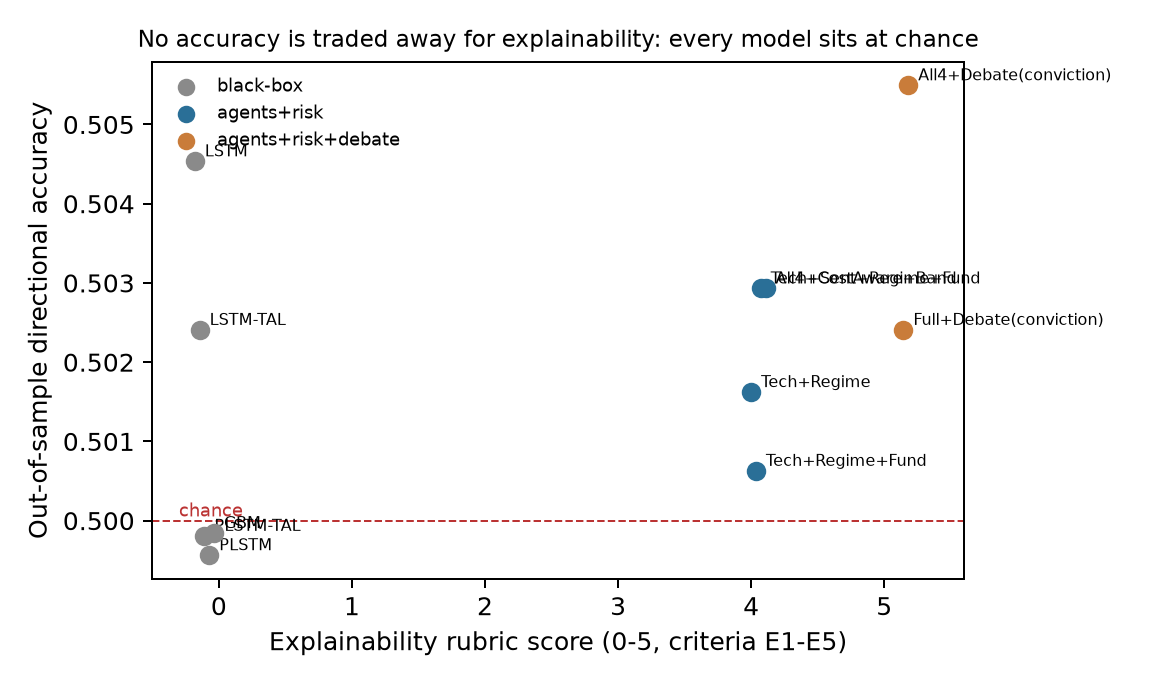
\includegraphics[width=0.8\linewidth]{accuracy_explainability.png}
\caption{Accuracy against explainability. Every model sits at chance.}
\end{figure}

The initial report proposed to quantify how much accuracy explainability costs. The answer is that it costs nothing here, because there is no accuracy to give up: black-box LSTMs and gradient boosting are at a coin flip, and so is every explainable configuration. In a low-signal market the binding constraint is signal, not interpretability, and the explainable design is strictly preferable -- it is the one that reveals the absence of signal.
\section{Discussion and limitations}
\begin{itemize}
\item \textbf{Statistical power.} The block-bootstrap test can reliably detect a Sharpe difference of about 1.0 over this window, not smaller; ``no significant difference'' is not ``proven identical''.
\item \textbf{Model scale.} No hosted frontier model was available; the comparison is 1.5B vs 3B open models. A frontier model could behave differently, though the 3B result gives no reason to expect a step change.
\item \textbf{Survivorship.} Both universes are today's large caps, which flatters Buy-and-Hold more than the agents.
\item \textbf{Fundamentals.} Disclosure-lagged but restated figures; annual frequency only; no valuation ratio.
\item \textbf{News coverage.} Google-News headlines for ten names; the extended universe has no sentiment.
\item \textbf{Data snapshot.} During the final evaluation a live-pipeline refresh overwrote the study's price cache; the newer Yahoo snapshot differs from the September one only by removing three phantom bars on NSE holidays (3 of 1,911 sessions). All strategies in each experiment are evaluated on one identical return series, and the cache is now write-protected in code.
\end{itemize}
\section{Conclusion}
The project set out to build an explainable multi-agent trading system for NSE equities and test whether it beats simple benchmarks. The system is built, tested and reproducible end to end. Under realistic Indian costs and honest statistics it does not beat Buy-and-Hold, on the original universe, on three times as many stocks, or on data that did not exist at the mid-semester review. None of the November additions changes that: a point-in-time fundamentals agent, a larger LLM, earnings-focused sentiment and cost-aware sizing. What survives is a regime-aware risk overlay that roughly halves drawdowns, and an explanation layer that is measurably faithful and was itself the instrument that diagnosed why the system behaves as it does. For a decision-support tool, a transparent ``no edge, but here is exactly why'' is a more useful result than an unexplained positive backtest.
\paragraph{Future work.} Intraday or event-time horizons where headline information has not yet been priced; point-in-time vendor fundamentals with valuation ratios; a frontier LLM for the debate; a cross-sectional (market-neutral) formulation that removes the market factor every per-name model currently fights.
\section*{Reproducibility}
\begin{footnotesize}\begin{verbatim}
cd nse_agents
.venv/bin/python -m pytest tests/ -q
.venv/bin/python scripts/final_fetch_prices.py        # extended prices
.venv/bin/python scripts/final_fetch_fundamentals.py  # annual reports
.venv/bin/python scripts/final_train_extended.py        # 30-name walk-forward
.venv/bin/python scripts/final_score_larger_llm.py      # Qwen2.5-3B scoring (MPS)
.venv/bin/python scripts/final_sentiment_studies.py     # earnings study, 1.5B vs 3B
.venv/bin/python scripts/final_run_ablation.py --experiment core --debate
.venv/bin/python scripts/final_run_ablation.py --experiment extended
.venv/bin/python scripts/final_explainability.py
.venv/bin/python scripts/final_make_report.py           # figures + this PDF
\end{verbatim}\end{footnotesize}
\begin{thebibliography}{9}
\bibitem{latif2024} S.~Latif, N.~Javaid, F.~Aslam, A.~Aldegheishem, N.~Alrajeh, S.~H.~Bouk. Enhanced prediction of stock markets using a novel deep learning model PLSTM-TAL in urbanized smart cities. \emph{Heliyon} 10(6):e27747, 2024.
\bibitem{lopezlira2023} A.~Lopez-Lira, Y.~Tang. Can ChatGPT forecast stock price movements? Return predictability and large language models. arXiv:2304.07619, 2023 (rev.\ 2025).
\bibitem{xiao2024} Y.~Xiao, E.~Sun, D.~Luo, W.~Wang. TradingAgents: Multi-agents LLM financial trading framework. arXiv:2412.20138, 2024.
\bibitem{an2022} B.~An, S.~Sun, R.~Wang. Deep reinforcement learning for quantitative trading: Challenges and opportunities. \emph{IEEE Intelligent Systems} 37(2):23--26, 2022.
\bibitem{muhammad2024} D.~Muhammad, I.~Ahmed, K.~Naveed, M.~Bendechache. An explainable deep learning approach for stock market trend prediction. \emph{Heliyon} 10(21):e40095, 2024.
\end{thebibliography}
\end{document}
